\chapter{Konstruktion der rotierenden Walzen (NB)}
\label{s:rotierendeWalzen}
Bevor das Experiment im Windkanal stattfinden kann, m"ussen die rotierenden Walzen f"ur den Stumpfk"orper konstruiert werden. Die Walzen sitzen am Ende des K"orpers, wie in \abb{fig:modelschema} gezeigt. Es sind drei unterschiedliche Walzenpaare entstanden: ein glattes Walzenpaar, ein gezahntes Walzenpaar mit einem duty cycle von 33\% und ein gezahntes Walzenpaar mit einem duty cycle von 50 \%.\\
%Die rotierenden Walzen sind jeweils auf einer Welle gelagert und werden von Elektromotoren angetrieben. Die Elektromotoren haben eine maximale Drehrate von 3650 Umdrehungenpro Minute und eine minimale Drehrate von um die 100 Umdrehungen pro Minute.

\begin{figure}[h]
	\centering
	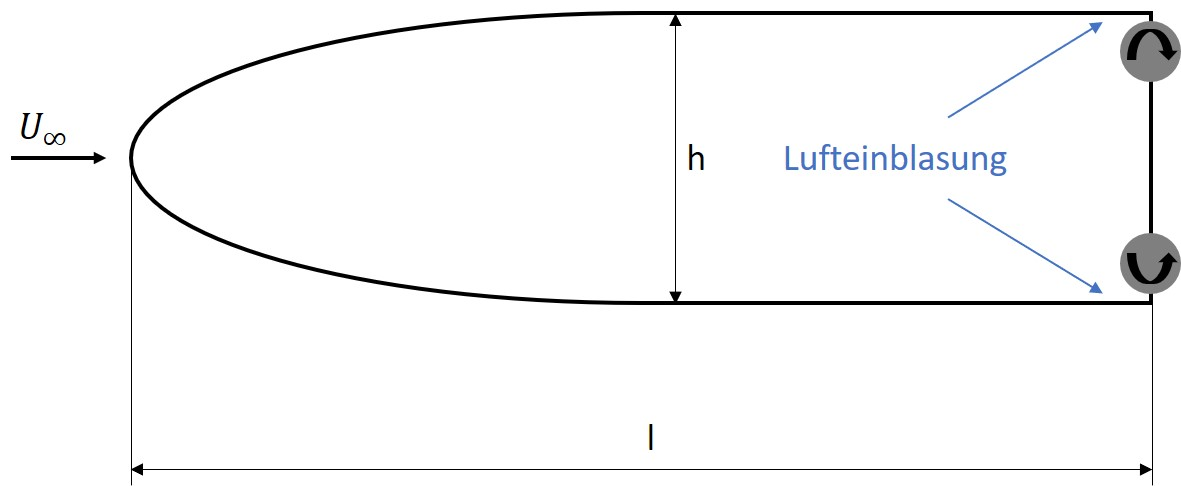
\includegraphics[width=0.8\textwidth]{ModellSchema.jpg}
	\caption{schematische Darstellung des Versuchsmodells}
	\label{fig:modelschema}
\end{figure}
Die rotierenden Walzen erf"ullen die Aufgabe, der gepulsten Einblasung in die Str"omung am Ende des Stumpfk"orpers.\\
Die Walzen bestehen aus einer Aluminium Innenewelle und einem mit Presspassung verbundenen Teflonrohr. In dem Teflonrohr ist die entscheidende Zahngeometire eingebracht. F"ur die Konstruktion des Teflonrohrs mussten folgende Aspekte betrachtet werden:
\begin{enumerate}
	\item Zahnform 
	\item Anzahl der Z"ahne
	\item Zahn"offnung 
\end{enumerate}

%----------------------------------------------------------------------------------
\section{Zahnform}
F"ur die Wahl einer Zahnform muss erst das auf die Str"omung aufgebrachte Signal festgelegt werden. Als Signale kommen daf"ur unterschiedliche Funktionen in Frage: Sinus-Funktion, Dirac-Impuls, Heaviside-Funktion usw..\\
%Die Zahnform hat Auswirkungen auf das gepulste Signal, das in die Str"omung eingef"uhrt wird. Als Grundlagen f"ur die Signalform wurden folgende mathematische Funktionen (\abb{fig:function}) betrachtet.\\
%\begin{figure}[h]
%	\centering
%	\begin{subfigure}[c]{0.5\textwidth}		
%		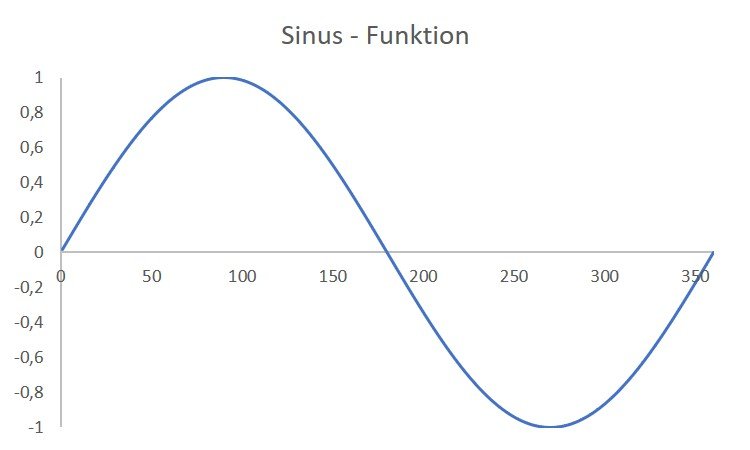
\includegraphics[width=1\textwidth]{Sinus.jpg}
%	\begin{subfigure}[c]{0.5\textwidth}
%		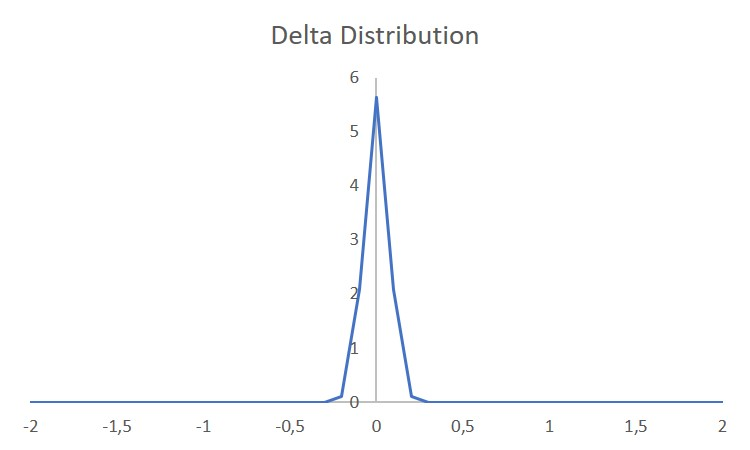
\includegraphics[width=1\textwidth]{DeltaDistribution.jpg}
%	\end{subfigure}
%	\begin{subfigure}[c]{0.5\textwidth}
%		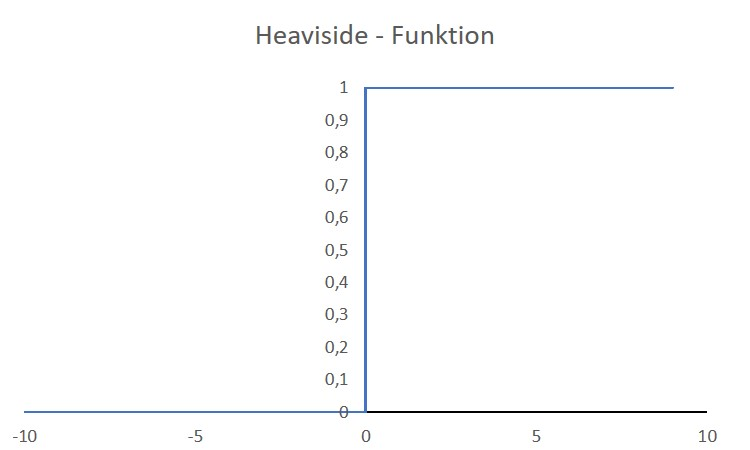
\includegraphics[width=1\textwidth]{Heaviside.jpg}
%	\end{subfigure}
%	\caption{mathematische Funktionen f"ur Zahnform}
%	\label{fig:function}
%\end{figure}\\
%F"ur die Sinus Funktion eignet sich eher eine andere Form der Str"omungsanregung, als die der drehenden Walzen. Diese kann besser "uber einen Null-Netto-Massenstrom-Jet-Aktuator \cite{Utturkar.2003} oder einen Lautsprecher dargestellt werden. Beide funktionieren "uber eine schwingende Membran, welche die Str"omung anregt.\\
%Ein Dirac-Impuls ist eine kurze Anregung der Str"omung. Die Zeit in der die Luft in die Str"omung eingeblasen wird, ist kurz im Vergleich zu der Zeit in der keine Anregung stattfindet. Damit k"onnte es zu einer nicht ausreichend gr\ss{}en Anregung kommen, die den gew"unschten Effekt nicht induziert.\\
%Eine Heaviside-Funktion stellt ein eindeutiges Signal dar, das entweder vollst"andig geschlossen oder ge"offnet ist. Somit ist eine klare Definition des Zustands m"oglich.\\
Bei der endg"ultigen Wahl eines Signals ist der fertigungstechnische Aspekt ein weiterer wichtiger Parameter, der in diesem Fall die Wahl des Signals entschieden hat. Als finales Wellendesign wurden die zwei Wellen aus \abb{fig:finalesdesign} gefertigt. Diese wurden gew"ahlt, da eine Fr"asbearbeitung des Teflonrohrs zu str"omungsmechanisch ung"unstigen Effekten gef"uhrt h"atte. Der Fr"aser hat immer eine endliche Breite, sodass die Str"omung durch die eventuell auftretenden minimalen Kanten zwischen den einzelnen Fr"asbahnen gest"ort werden k"onnte. Somit wurde sich f"ur eine Fertigung auf der Drehmaschine entschieden. Dabei wurden die Zahnt"aler "uber eine exzentrische Einspannung erreicht. Die Wahl f"ur zwei Wellen wird im Folgenden n"aher betrachtet.
\begin{figure}[h]
	\centering
	\begin{subfigure}[c]{0.4\textwidth}		
		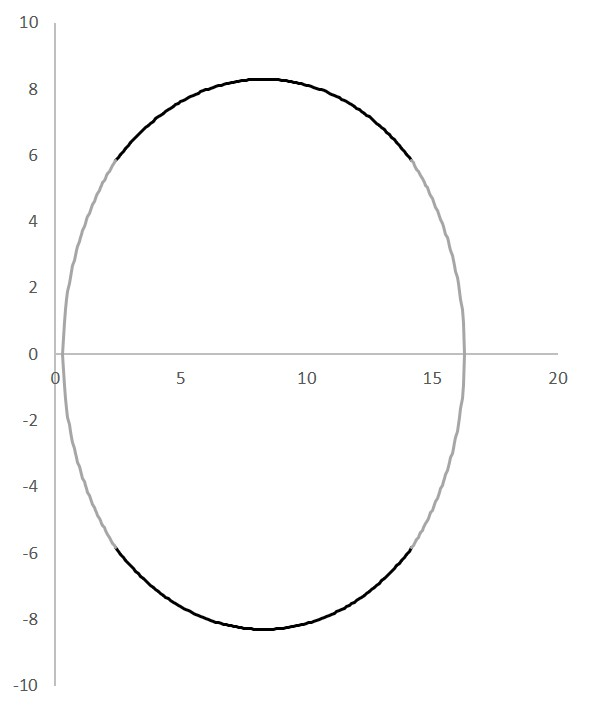
\includegraphics[width=0.8\textwidth]{Walze1Graphik.jpg}
	\end{subfigure}
	\begin{subfigure}[c]{0.4\textwidth}
		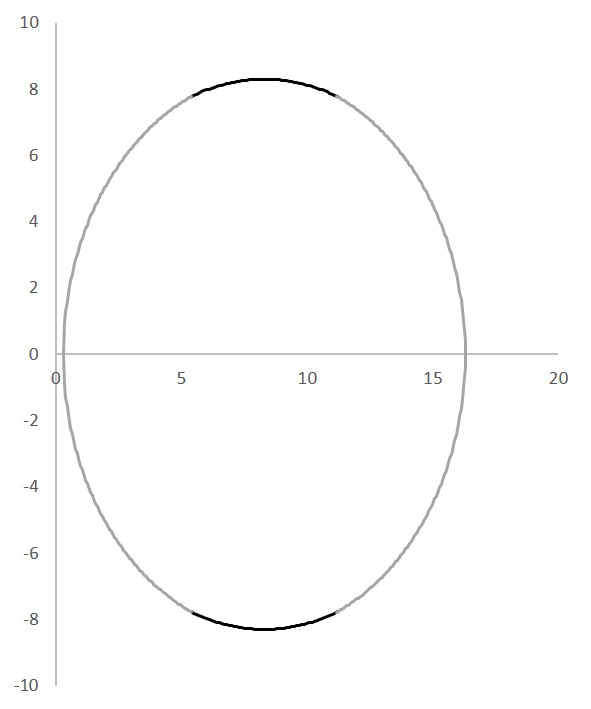
\includegraphics[width=0.8\textwidth]{Walze2Graphik.jpg}
	\end{subfigure}
	\caption{Querschnitt durch die finalen Walzen}
	\label{fig:finalesdesign}
\end{figure}\\

Die Walzenformen lassen sich "uber mehrere Kreisfunktionen auf unterschiedlichen Intervallen darstellen (verschiedene Farben in \abb{fig:finalesdesign}). Die linke Walze kann beschrieben werden "uber \glg{eq:Walze1}.
\begin{align}
	{f_1(x)}=\pm\sqrt{9,15^{2}-(x-9,45)^{2}}\,\,\,\,&x\in[0,3; 2,42] \label{eq:Walze1}\\
	{g_1(x)}=\pm\sqrt{8,3^{2}-(x-8,3)^{2}}\,\,\,\,&x\in[2,42; 14,18] \nonumber\\
	{h_1(x)}=\pm\sqrt{9,15^{2}-(x-7,15)^{2}}\,\,\,\,&x\in[14,18; 16] \nonumber
\end{align}\\
Die rechte Walze kann beschrieben werden "uber \glg{eq:Walze2}.
\begin{align}
	{f_2(x)}=\pm\sqrt{8,48^{2}-(x-8,78)^{2}}\,\,\,\,&x\in[0,3; 5,39] \label{eq:Walze2}\\
	{g_2(x)}=\pm\sqrt{8,3^{2}-(x-8,3)^{2}}\,\,\,\,&x\in[5,39; 10,61] \nonumber\\
	{h_2(x)}=\pm\sqrt{8,48^{2}-(x-7,82)^{2}}\,\,\,\,&x\in[10,61; 16] \nonumber
\end{align}\\
Aus der Form der Walzen, die die Zahnform darstellen, l"asst sich r"uckwirkend auf die Signalform schlie\ss{}en. Das Signal ist in \abb{fig:spaltverlauf} dargestellt. Ein Wert von \SI{0,3}{\milli\meter} entspricht dabei einem offenen Signal, d.h. es wird Luft in den Spalt eingeblasen. Bei einem Wert von \SI{0}{\milli\meter} findet keine Einblasung statt. In den Graphiken ist ein Signalverlauf f"ur eine Viertelumdrehung der Walze dargestellt. Aufgrund von Symmetrie folgt im weiteren ein spiegelverkehrter Verlauf und danach eine periodische Fortsetzung, wie in \abb{fig:signal} dargestellt.
\begin{figure}[h]
	\centering
	\begin{subfigure}[c]{0.7\textwidth}		
		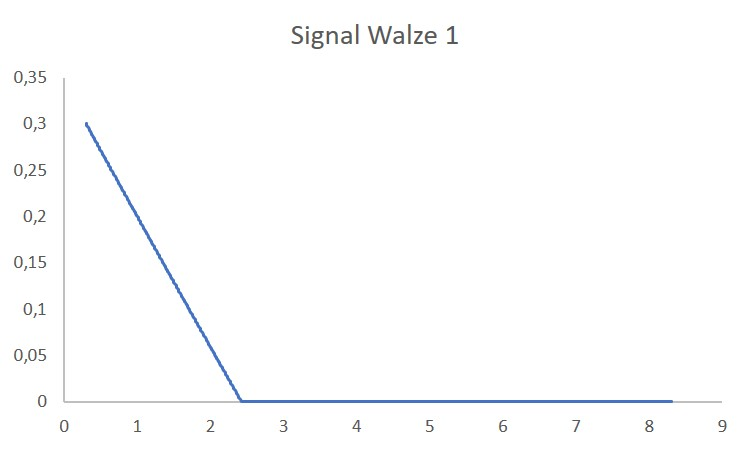
\includegraphics[width=1\textwidth]{Spaltverlauf1.jpg}
	\end{subfigure}
	\begin{subfigure}[c]{0.7\textwidth}
		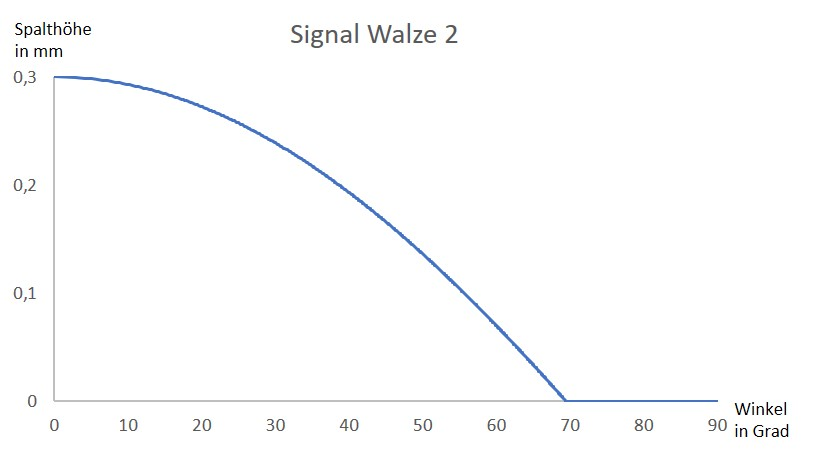
\includegraphics[width=1\textwidth]{Spaltverlauf2.jpg}
	\end{subfigure}
	\caption{Signalverlauf der Walzen}
	\label{fig:spaltverlauf}
\end{figure}

\begin{figure}[h]
	\centering
	\begin{subfigure}[c]{0.5\textwidth}		
		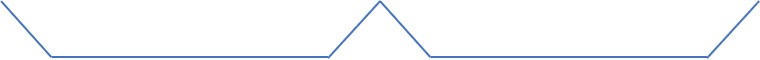
\includegraphics[width=1.2\textwidth]{SignalWalze1.jpg}
	\end{subfigure}
	\begin{subfigure}[c]{0.5\textwidth}
		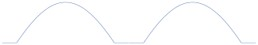
\includegraphics[width=1.2\textwidth]{SignalWalze2.jpg}
	\end{subfigure}
	\caption{Periodische Signale der Walzen}
	\label{fig:signal}
\end{figure}


%--------------------------------------------------------------------------------------
\newpage
\section{Anzahl der Z"ahne}
Als zweites wird im Folgenden auf die Entscheidung der Anzahl der Z"ahne detailierter eingegangen. Ein ausschlaggebender Punkt ist dabei, dass die Einblasung mit einer Frequenz in Umgebung der Abl"osefrequenz der Str"omung durchgef"uhrt wird, besonders interessant ist eine Frequenz leicht oberhalb der Abl"osefrequenz (siehe \cite{Oswald.2017}). Au\ss{}erdem soll die Drehzahl der Elektromotoren nicht "uber- bzw. unterschritten werden. Diese liegt maximal bei 3650 Umdrehungen pro Minute und minimal bei 100 Umdrehungen pro Minute.\\
Die Abl"osefrequenz der Str"omung kann "uber die dimensionslose Strouhal-Zahl mit \glg{eq:Str} bestimmt werden. Wenn diese nach der gew"unschten Variable umgestellt wird (siehe \glg{eq:nachfumgestellt}) und die gegebenen Werte aus \tab{tab:Modellwerte} eingesetzt werden, kann die Frequenz
\begin{align}
	{f}=\frac{Str*U_{\infty}}{D}
		=\frac{0,23*\SI{15}{\meter\per\second}}{\SI{0,0534}{\meter}}
		=\SI{64,61}{\hertz}
		\label{eq:nachfumgestellt}
\end{align}
berechnet werden.
\begin{table}[h!]
	\centering
	\begin{tabular}{lr}
		\toprule
		Parameter & Wert\\
		\midrule
		Strouhal-Zahl & 0,23\\
		Anstr"omgeschwindigkeit & \SI{15}{\meter\per\second}\\
		Profildicke & \SI{53,4}{\milli\meter}\\
		\bottomrule
	\end{tabular}
	\caption{Modellwerte f"ur Frequenzberechnung}
	\label{tab:Modellwerte}
\end{table}\\
Aus der Frequenz, die mindestens erreicht werden soll, kann nun berechnet werden, wie schnell sich die Walze mit welcher Z"ahnezahl drehen muss. Das Ergebnis f"ur unterschiedliche Z"ahne findet sich in \tab{tab:zahnezahl}.\\
\begin{table}[h]
	\centering
	\begin{tabular}{lrr}
		\toprule
		Anzahl der Z"ahne & Drehgeschwindigkeit der Welle [Hz] & Drehgeschwindigkeit der Welle [rpm]\\
		\midrule
		1 & 64,61 & 3876,6\\
		2 & 32,30 & 1938,0\\
		4 & 16,15 & 969,0\\
		6 & 10,77 & 646,2\\
		8 & 8,08 & 484,8\\
		10 & 6,46 & 387,6\\
		\bottomrule
	\end{tabular}\\
	\caption{Z"ahnezahlen mit zugeh"origen Frequenzen}
	\label{tab:zahnezahl}
\end{table}

Aufgrund von Symmetrie und um dem m"oglichen entstehen einer Unwucht entgegen zu wirken, wurde sich f"ur eine gerade Z"ahnezahl entschieden. Da eine ausreichend gro\ss{}e L"ucke ben"otigt wird, um den Z"ahnen einen effektiven Luftaussto\ss{} zu gew"ahrleisten, wurde sich f"ur eine Z"ahnezahl von zwei pro Walze entschieden.\\

%-----------------------------------------------------------------------------------
\section{Zahn"offnung}
Als dritten Aspekt der Zahngestaltung wird im Folgendem die Zahn"offnung betrachtet. Es wurden zwei Walzen mit zwei unterschiedlichen duty cyclen gefertigt. Die Berechnungen des duty cycles f"ur die erste Walze ist "uber Integration von \glg{eq:Walze1} und f"ur die zweite Walze von \glg{eq:Walze2} an einer Viertelwalze erfolgt. F"ur die Berechnungen wird das MATLAB Skript aus \abb{fig:Integrationsskript} verwendet. Somit ergibt sich f"ur die erste Walze ein duty cycle von 33\% und f"ur die zweite von 50\%.
\begin{figure}[h]
	\centering
	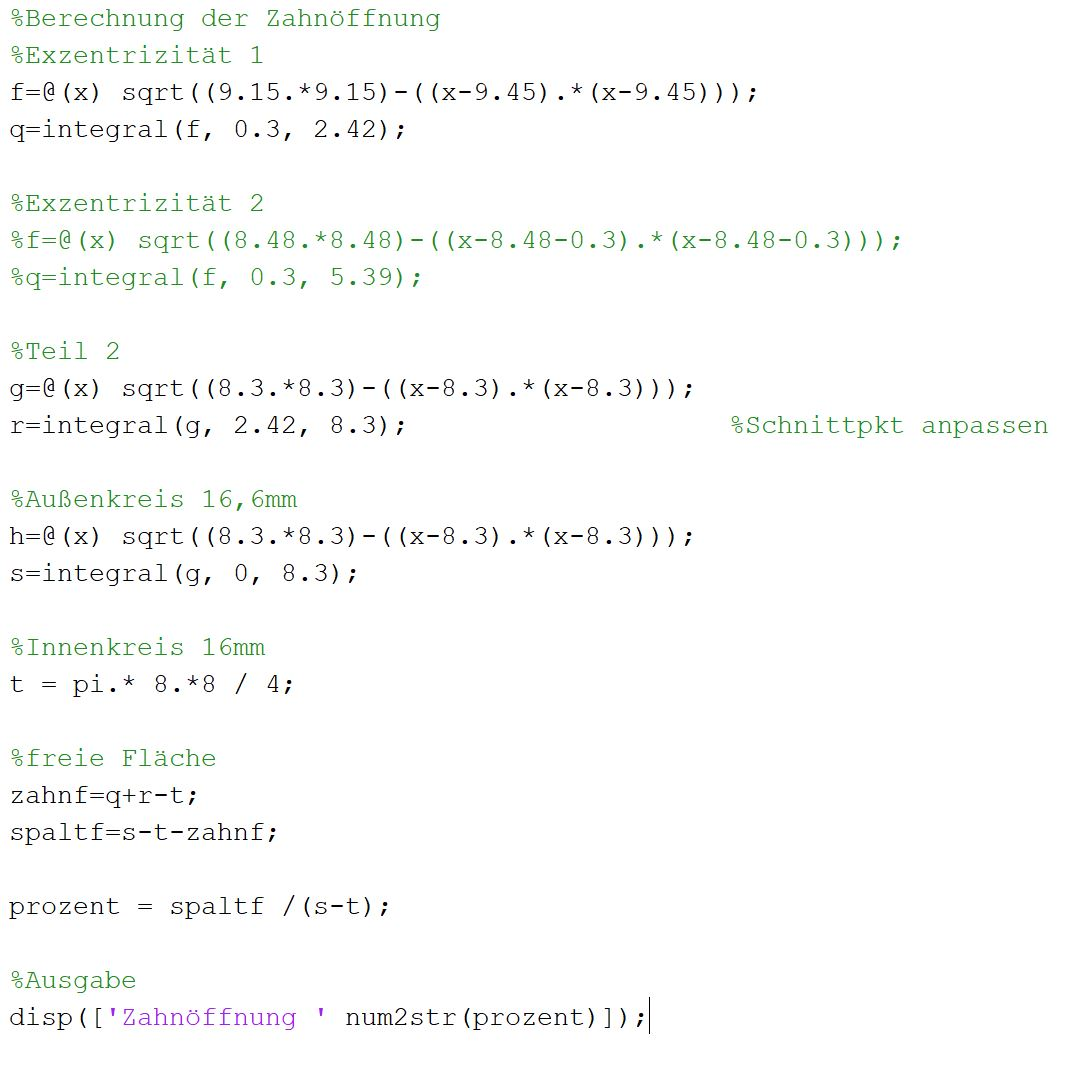
\includegraphics[width=0.8\textwidth]{Integrationsskript.jpg}
	\caption{MATLAB Skript zur Berechnung der Zahn"offnung}
	\label{fig:Integrationsskript}
\end{figure}\\



